% Options for packages loaded elsewhere
% Options for packages loaded elsewhere
\PassOptionsToPackage{unicode}{hyperref}
\PassOptionsToPackage{hyphens}{url}
%
\documentclass[
  english,
  russian,
  12pt,
  a4paper,
  DIV=11,
  numbers=noendperiod]{scrreprt}
\usepackage{xcolor}
\usepackage{amsmath,amssymb}
\setcounter{secnumdepth}{5}
\usepackage{iftex}
\ifPDFTeX
  \usepackage[T1]{fontenc}
  \usepackage[utf8]{inputenc}
  \usepackage{textcomp} % provide euro and other symbols
\else % if luatex or xetex
  \usepackage{unicode-math} % this also loads fontspec
  \defaultfontfeatures{Scale=MatchLowercase}
  \defaultfontfeatures[\rmfamily]{Ligatures=TeX,Scale=1}
\fi
\usepackage{lmodern}
\ifPDFTeX\else
  % xetex/luatex font selection
\fi
% Use upquote if available, for straight quotes in verbatim environments
\IfFileExists{upquote.sty}{\usepackage{upquote}}{}
\IfFileExists{microtype.sty}{% use microtype if available
  \usepackage[]{microtype}
  \UseMicrotypeSet[protrusion]{basicmath} % disable protrusion for tt fonts
}{}
\usepackage{setspace}
% Make \paragraph and \subparagraph free-standing
\makeatletter
\ifx\paragraph\undefined\else
  \let\oldparagraph\paragraph
  \renewcommand{\paragraph}{
    \@ifstar
      \xxxParagraphStar
      \xxxParagraphNoStar
  }
  \newcommand{\xxxParagraphStar}[1]{\oldparagraph*{#1}\mbox{}}
  \newcommand{\xxxParagraphNoStar}[1]{\oldparagraph{#1}\mbox{}}
\fi
\ifx\subparagraph\undefined\else
  \let\oldsubparagraph\subparagraph
  \renewcommand{\subparagraph}{
    \@ifstar
      \xxxSubParagraphStar
      \xxxSubParagraphNoStar
  }
  \newcommand{\xxxSubParagraphStar}[1]{\oldsubparagraph*{#1}\mbox{}}
  \newcommand{\xxxSubParagraphNoStar}[1]{\oldsubparagraph{#1}\mbox{}}
\fi
\makeatother


\usepackage{longtable,booktabs,array}
\usepackage{calc} % for calculating minipage widths
% Correct order of tables after \paragraph or \subparagraph
\usepackage{etoolbox}
\makeatletter
\patchcmd\longtable{\par}{\if@noskipsec\mbox{}\fi\par}{}{}
\makeatother
% Allow footnotes in longtable head/foot
\IfFileExists{footnotehyper.sty}{\usepackage{footnotehyper}}{\usepackage{footnote}}
\makesavenoteenv{longtable}
\usepackage{graphicx}
\makeatletter
\newsavebox\pandoc@box
\newcommand*\pandocbounded[1]{% scales image to fit in text height/width
  \sbox\pandoc@box{#1}%
  \Gscale@div\@tempa{\textheight}{\dimexpr\ht\pandoc@box+\dp\pandoc@box\relax}%
  \Gscale@div\@tempb{\linewidth}{\wd\pandoc@box}%
  \ifdim\@tempb\p@<\@tempa\p@\let\@tempa\@tempb\fi% select the smaller of both
  \ifdim\@tempa\p@<\p@\scalebox{\@tempa}{\usebox\pandoc@box}%
  \else\usebox{\pandoc@box}%
  \fi%
}
% Set default figure placement to htbp
\def\fps@figure{htbp}
\makeatother



\ifLuaTeX
\usepackage[bidi=basic,provide=*]{babel}
\else
\usepackage[bidi=default,provide=*]{babel}
\fi
% get rid of language-specific shorthands (see #6817):
\let\LanguageShortHands\languageshorthands
\def\languageshorthands#1{}


\setlength{\emergencystretch}{3em} % prevent overfull lines

\providecommand{\tightlist}{%
  \setlength{\itemsep}{0pt}\setlength{\parskip}{0pt}}



 
\usepackage[backend=biber,langhook=extras,autolang=other*]{biblatex}
\addbibresource{bib/cite.bib}

\usepackage[]{csquotes}

\usepackage{indentfirst}
\usepackage{float}
\floatplacement{figure}{H}
\IfFileExists{plex-otf.sty}{
  %% Full TeXlive
  \usepackage[math,RM={Scale=0.94},SS={Scale=0.94},SScon={Scale=0.94},TT={Scale=MatchLowercase,FakeStretch=0.9},DefaultFeatures={Ligatures=Common}]{plex-otf}
}{
  %% TinyTeX
  \usepackage{libertine}
}
\KOMAoption{captions}{tableheading}
\makeatletter
\@ifpackageloaded{caption}{}{\usepackage{caption}}
\AtBeginDocument{%
\ifdefined\contentsname
  \renewcommand*\contentsname{Содержание}
\else
  \newcommand\contentsname{Содержание}
\fi
\ifdefined\listfigurename
  \renewcommand*\listfigurename{Список иллюстраций}
\else
  \newcommand\listfigurename{Список иллюстраций}
\fi
\ifdefined\listtablename
  \renewcommand*\listtablename{Список таблиц}
\else
  \newcommand\listtablename{Список таблиц}
\fi
\ifdefined\figurename
  \renewcommand*\figurename{Рисунок}
\else
  \newcommand\figurename{Рисунок}
\fi
\ifdefined\tablename
  \renewcommand*\tablename{Таблица}
\else
  \newcommand\tablename{Таблица}
\fi
}
\@ifpackageloaded{float}{}{\usepackage{float}}
\floatstyle{ruled}
\@ifundefined{c@chapter}{\newfloat{codelisting}{h}{lop}}{\newfloat{codelisting}{h}{lop}[chapter]}
\floatname{codelisting}{Список}
\newcommand*\listoflistings{\listof{codelisting}{Листинги}}
\makeatother
\makeatletter
\makeatother
\makeatletter
\@ifpackageloaded{caption}{}{\usepackage{caption}}
\@ifpackageloaded{subcaption}{}{\usepackage{subcaption}}
\makeatother
\usepackage{bookmark}
\IfFileExists{xurl.sty}{\usepackage{xurl}}{} % add URL line breaks if available
\urlstyle{same}
\hypersetup{
  pdftitle={Лабораторная работа №4},
  pdfauthor={Данилова Анастасия Сергеевна},
  pdflang={ru-RU},
  hidelinks,
  pdfcreator={LaTeX via pandoc}}


\title{Лабораторная работа №4}
\usepackage{etoolbox}
\makeatletter
\providecommand{\subtitle}[1]{% add subtitle to \maketitle
  \apptocmd{\@title}{\par {\large #1 \par}}{}{}
}
\makeatother
\subtitle{Простейший вариант}
\author{Данилова Анастасия Сергеевна}
\date{}
\begin{document}
\maketitle

\renewcommand*\contentsname{Содержание}
{
\setcounter{tocdepth}{1}
\tableofcontents
}
\listoffigures
\listoftables

\setstretch{1.5}
\chapter{Цель
работы}\label{ux446ux435ux43bux44c-ux440ux430ux431ux43eux442ux44b}

Цель данной работы научиться оформлять изображения в тексте, а также
правильно работать с ссылками.

\chapter{Задание}\label{ux437ux430ux434ux430ux43dux438ux435}

Повторить приведенные примеры, а также выполнить упражнения:

\begin{itemize}
\tightlist
\item
  Попробуйте вставить созданное вами изображение, заменив
  \enquote{стандартные} изображения, которые мы использовали в
  демонстрации.
\item
  Узнайте, что вы можете сделать, используя клавиши height, width, angle
  и scale.
\item
  Используйте клавишу width, чтобы задать размер графического
  изображения относительно textwidth, а другого графического изображения
  - относительно linewidth. Посмотрите, как они ведут себя с опцией
  twocolumn или без нее.
\item
  Используйте lipsum, чтобы провести достаточно длинную демонстрацию, а
  затем попробуйте разместить плавающие изображения, используя разные
  спецификаторы положения. Как взаимодействуют разные спецификаторы?
\item
  Попробуйте добавить в тестовый документ новые пронумерованные части
  (разделы, подразделы, списки с нумерацией) и выясните, сколько
  запусков требуется для выполнения команд label.
\item
  Добавьте несколько плавающих изображений и посмотрите, что произойдет,
  если вы поставите label перед caption, а не после; можете ли вы
  предсказать результат?
\item
  Что произойдет, если вы поставите label для уравнения после
  end\{уравнения\}?
\end{itemize}

\chapter{Теоретическое
введение}\label{ux442ux435ux43eux440ux435ux442ux438ux447ux435ux441ux43aux43eux435-ux432ux432ux435ux434ux435ux43dux438ux435}

Вы можете использовать файлы формата EPS, PNG, JPG и PDF. Если у вас
есть несколько версий графического изображения, вы можете написать,
например, example-image.png. (Пакет graphicx попытается угадать
расширение, если вы его не укажете). Команда includegraphics имеет
множество опций для управления размером и формой включаемых изображений,
а также для обрезки материала. Некоторые из них часто используются,
поэтому о них стоит знать. Наиболее очевидная вещь, которую нужно
задать, - это ширина или высота изображения, которые часто задаются
относительно textwidth или linewidth и textheight. Разница между
textwidth и linewidth незначительна, и часто результат один и тот же.
textwidth - это ширина текстового блока на физической странице, тогда
как linewidth - это текущая ширина, которая может отличаться на
локальном уровне (разница наиболее очевидна опция class twocolumn).
LaTeX автоматически масштабирует изображение таким образом, чтобы
соотношение сторон оставалось правильным. Более подробно про Unix см. в
\autocite{kotelnikov_chebotaev_book_latex2_ru,lvovsky_book_latex_ru}.

\chapter{Выполнение лабораторной
работы}\label{ux432ux44bux43fux43eux43bux43dux435ux43dux438ux435-ux43bux430ux431ux43eux440ux430ux442ux43eux440ux43dux43eux439-ux440ux430ux431ux43eux442ux44b}

Попробуем вставить изображение по центру и укажем высоту 2.

\begin{figure}

\centering{

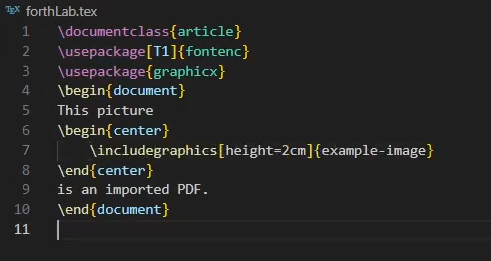
\includegraphics[width=0.7\linewidth,height=\textheight,keepaspectratio]{image/1.png}

}

\caption{\label{fig-001}Простой пример}

\end{figure}%

\begin{figure}

\centering{


\includegraphics[width=0.7\linewidth,height=\textheight,keepaspectratio]{image/2.png}

}

\caption{\label{fig-002}Результат}

\end{figure}%

Указываем размер картинки по высоте и ширине. В данном случае разница
хорошо видна, но обычно, она не так заметно. Более яркое различие будет,
если использовать параметр twocolumn. (рис.~\ref{fig-004}).

\begin{figure}

\centering{

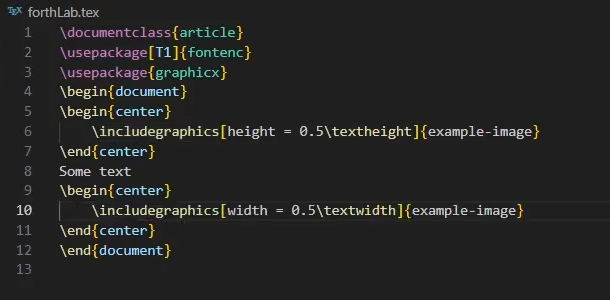
\includegraphics[width=0.7\linewidth,height=\textheight,keepaspectratio]{image/3.png}

}

\caption{\label{fig-003}Второй пример}

\end{figure}%

\begin{figure}

\centering{


\includegraphics[width=0.7\linewidth,height=\textheight,keepaspectratio]{image/4.png}

}

\caption{\label{fig-004}Результат изменения размеров}

\end{figure}%

Теперь попробуем обрезать картинку.

\begin{figure}

\centering{

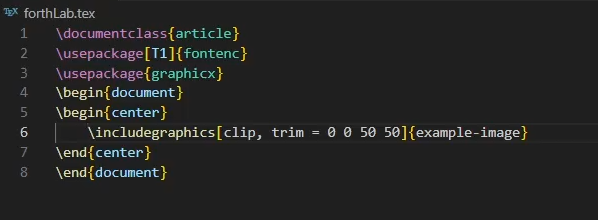
\includegraphics[width=0.7\linewidth,height=\textheight,keepaspectratio]{image/5.png}

}

\caption{\label{fig-005}Clip и trim}

\end{figure}%

Посмотрим на результат (рис.~\ref{fig-006}).

\begin{figure}

\centering{

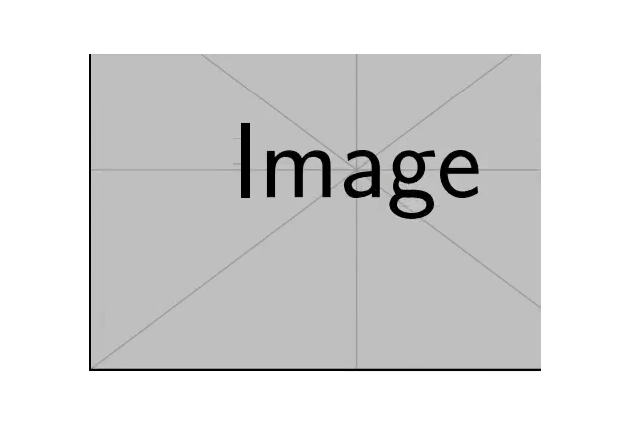
\includegraphics[width=0.7\linewidth,height=\textheight,keepaspectratio]{image/6.png}

}

\caption{\label{fig-006}Результат}

\end{figure}%

Обычно изображения могут двигаться свободно по документу. Они называются
плавающими. Поэтому мы будем использовать некоторые параметры, чтобы
разместить объект там, где мы хотим.

\begin{figure}

\centering{

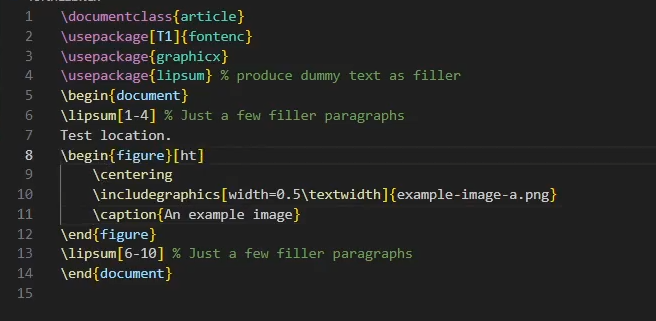
\includegraphics[width=0.7\linewidth,height=\textheight,keepaspectratio]{image/7.png}

}

\caption{\label{fig-007}Спецификаторы}

\end{figure}%

Есть несколько видов спецификаторов:

• h \enquote*{здесь} (если возможно) • t верх страницы • b низ страницы
• p выделенная страница для плавающих

\begin{figure}

\centering{

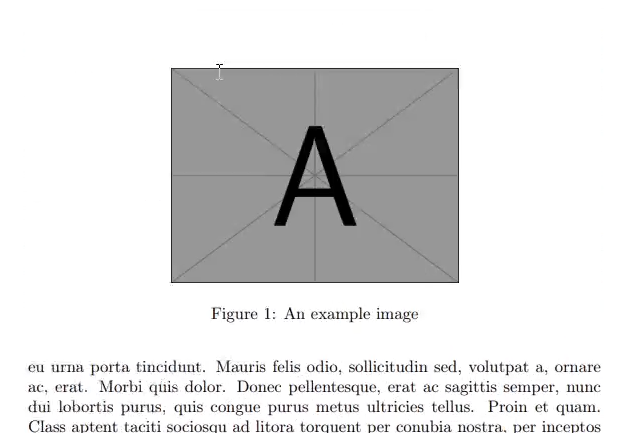
\includegraphics[width=0.7\linewidth,height=\textheight,keepaspectratio]{image/8.png}

}

\caption{\label{fig-008}ht}

\end{figure}%

Еще один вид - это H (дословный перевод \enquote{абсолютно точно
здесь}). Обычно, его не рекомендуется использовать, так как могут
образоваться большие пробелмы на странице.

\begin{figure}

\centering{

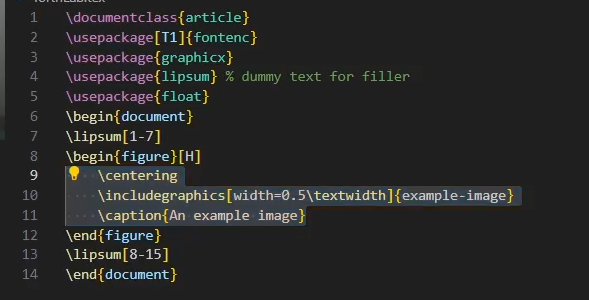
\includegraphics[width=0.7\linewidth,height=\textheight,keepaspectratio]{image/9.png}

}

\caption{\label{fig-009}H}

\end{figure}%

\begin{figure}

\centering{

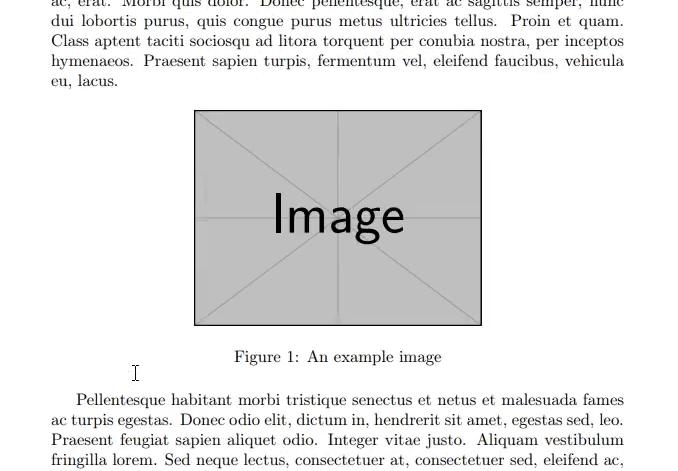
\includegraphics[width=0.7\linewidth,height=\textheight,keepaspectratio]{image/10.png}

}

\caption{\label{fig-010}Как выглядит H}

\end{figure}%

Также могут понадобиться другие типы для плавающих объектов. Они
встраиваются отдельно с помощью пакета trivfloat.

\begin{figure}

\centering{

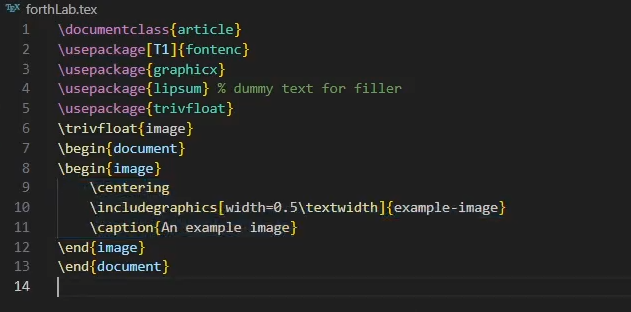
\includegraphics[width=0.7\linewidth,height=\textheight,keepaspectratio]{image/11.png}

}

\caption{\label{fig-011}Расположение объекта}

\end{figure}%

\begin{figure}

\centering{

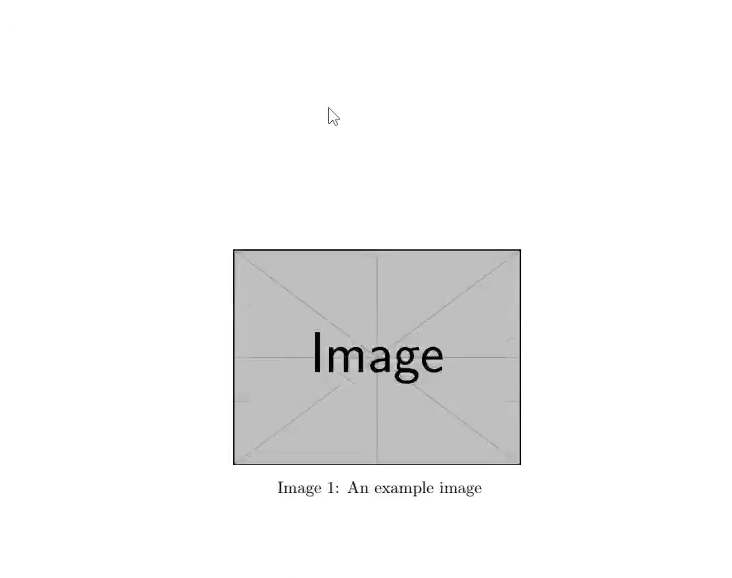
\includegraphics[width=0.7\linewidth,height=\textheight,keepaspectratio]{image/12.png}

}

\caption{\label{fig-012}Результат расположения}

\end{figure}%

Теперь перейдем к ссылкам.

\begin{figure}

\centering{

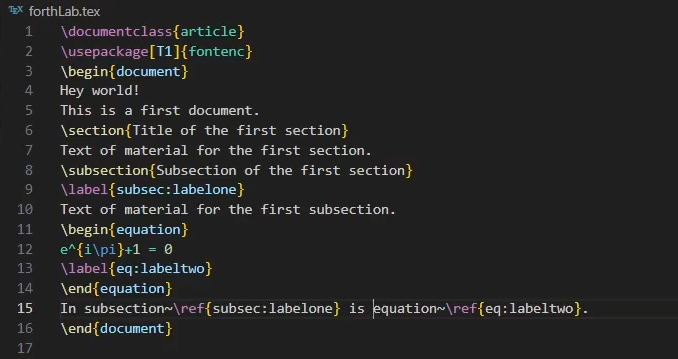
\includegraphics[width=0.7\linewidth,height=\textheight,keepaspectratio]{image/13.png}

}

\caption{\label{fig-013}Ссылки}

\end{figure}%

Для ссылок мы также подключаем новый пакет. А также обратим внимание,
что для того, чтобы ссылка отображалась, документ нужно сконвертировать
минимум дважды.

\begin{figure}

\centering{

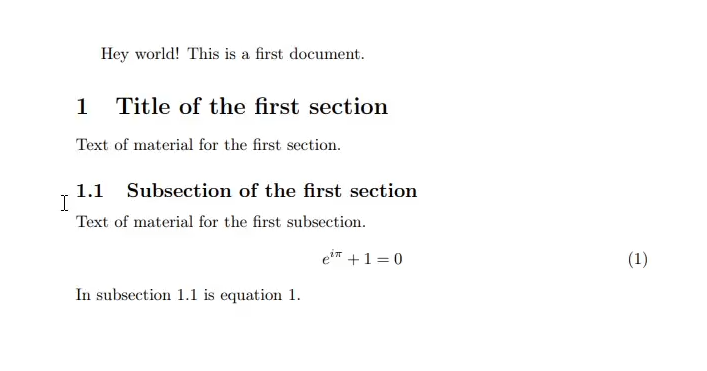
\includegraphics[width=0.7\linewidth,height=\textheight,keepaspectratio]{image/14.png}

}

\caption{\label{fig-014}Пример ссылки}

\end{figure}%

Важно обращать внимание на расположение пакета. Он должен прогружаться
после всех остальных.

\begin{figure}

\centering{

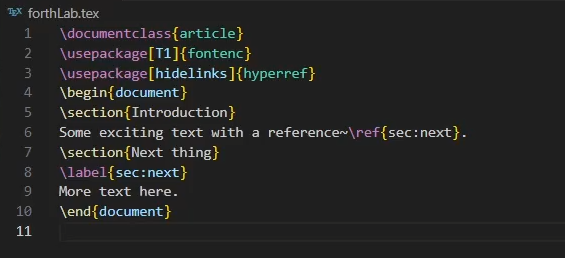
\includegraphics[width=0.7\linewidth,height=\textheight,keepaspectratio]{image/15.png}

}

\caption{\label{fig-015}Пакет hyperref}

\end{figure}%

\begin{figure}

\centering{

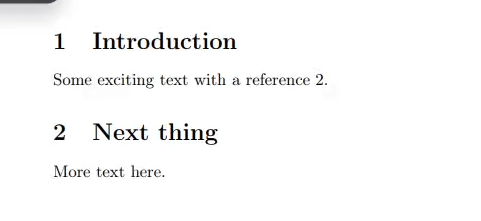
\includegraphics[width=0.7\linewidth,height=\textheight,keepaspectratio]{image/16.png}

}

\caption{\label{fig-016}Результат hyperref}

\end{figure}%

Теперь перейдем к упражнениям. В первом нам нужно было добавить свою
картинку.

\begin{figure}

\centering{

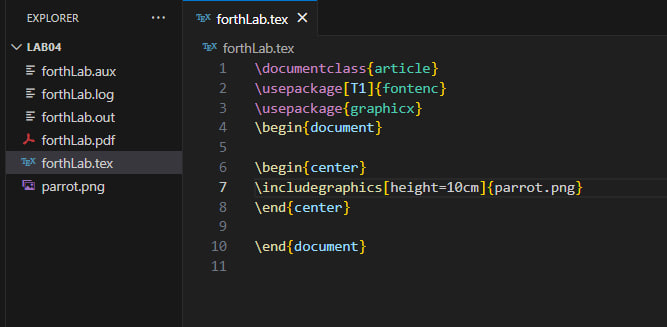
\includegraphics[width=0.7\linewidth,height=\textheight,keepaspectratio]{image/17.jpg}

}

\caption{\label{fig-017}Свое изображение}

\end{figure}%

\begin{figure}

\centering{

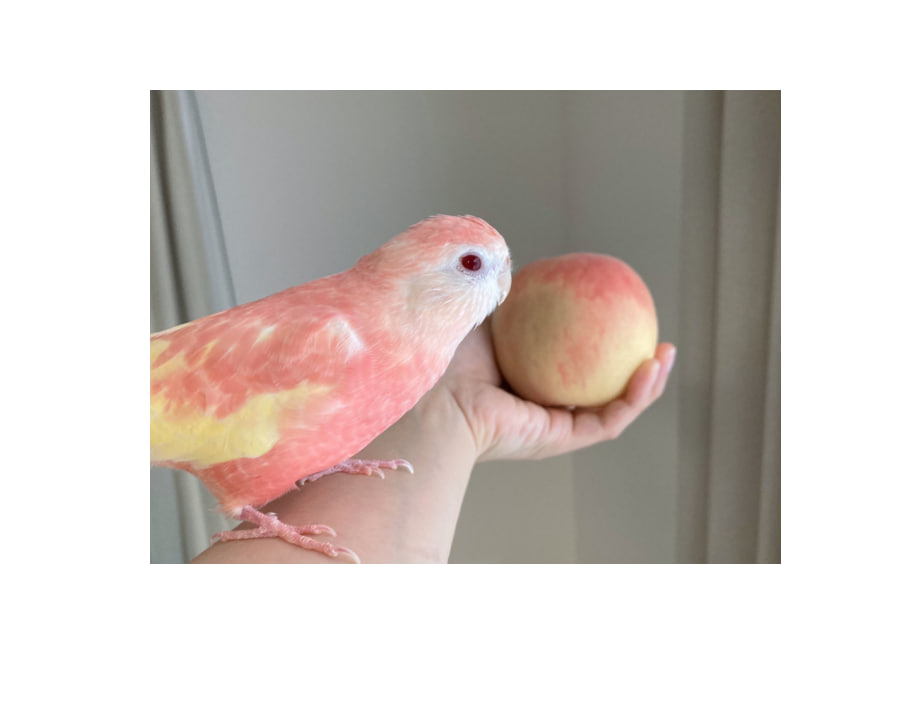
\includegraphics[width=0.7\linewidth,height=\textheight,keepaspectratio]{image/18.jpg}

}

\caption{\label{fig-018}Результат вывода}

\end{figure}%

Далее нужно было попробовать отредактировать это изображение с помощью
некоторых команд. Так как высоту и ширину мы уже рассматривали ранее, я
решила попробовать scale и angle.

\begin{figure}

\centering{

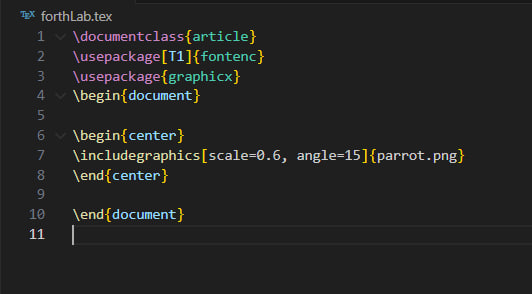
\includegraphics[width=0.7\linewidth,height=\textheight,keepaspectratio]{image/19.jpg}

}

\caption{\label{fig-019}Новые изменения}

\end{figure}%

\begin{figure}

\centering{

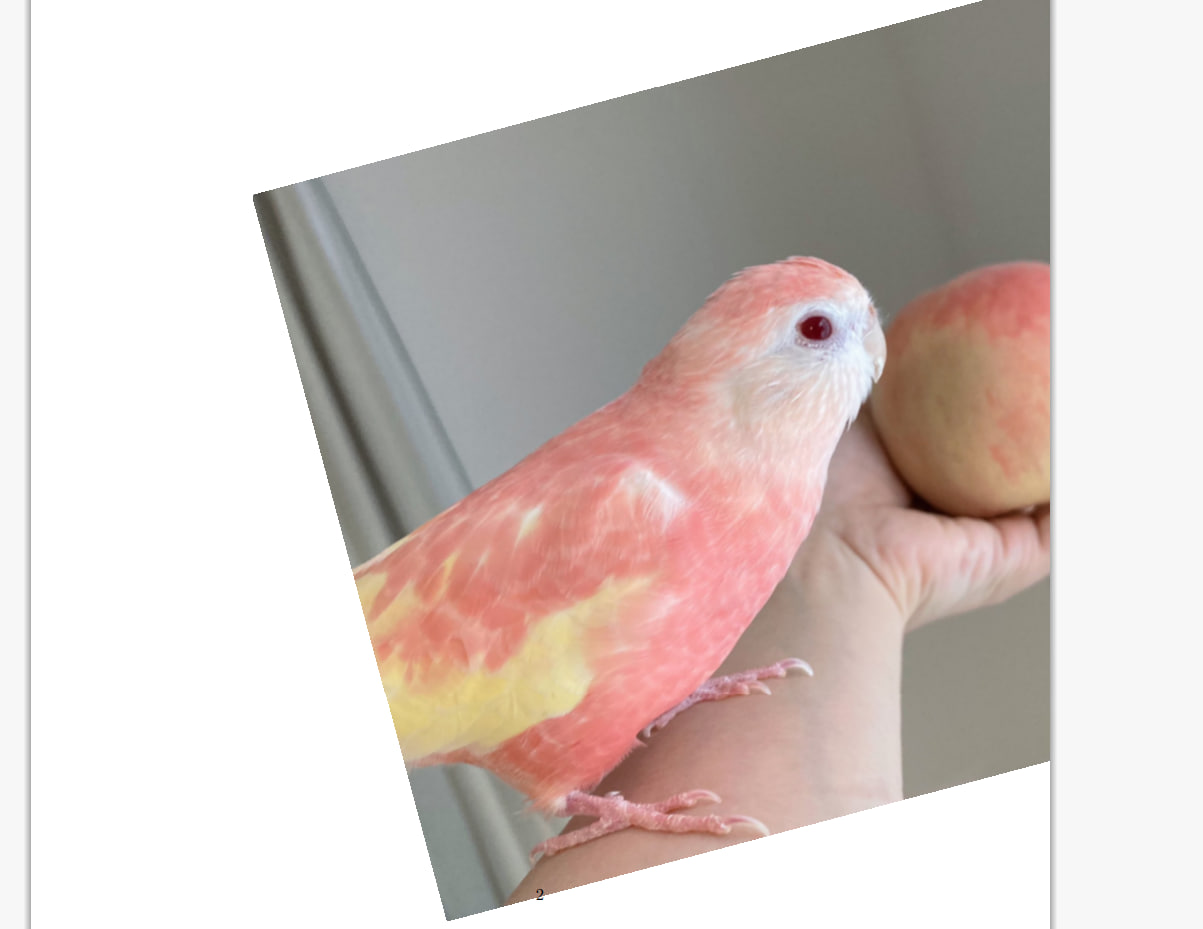
\includegraphics[width=0.7\linewidth,height=\textheight,keepaspectratio]{image/20.jpg}

}

\caption{\label{fig-020}Перевернутое и увеличенное изображение}

\end{figure}%

Теперь смотрим, как поведут себя textwidth и linewidth, если режим
одноколоночный и двуколоночный.

\begin{figure}

\centering{

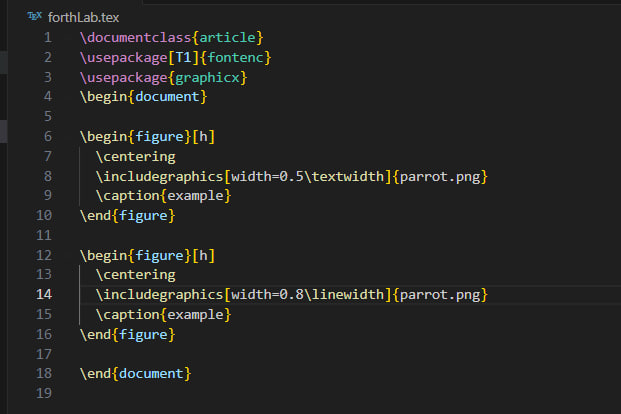
\includegraphics[width=0.7\linewidth,height=\textheight,keepaspectratio]{image/21.jpg}

}

\caption{\label{fig-021}Одна колонка}

\end{figure}%

Изображения одинакового размера

\begin{figure}

\centering{

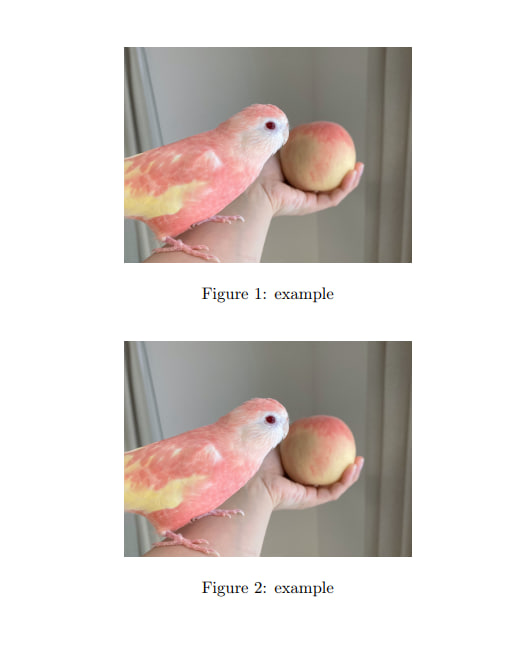
\includegraphics[width=0.7\linewidth,height=\textheight,keepaspectratio]{image/22.jpg}

}

\caption{\label{fig-022}Одна колонка}

\end{figure}%

\begin{figure}

\centering{

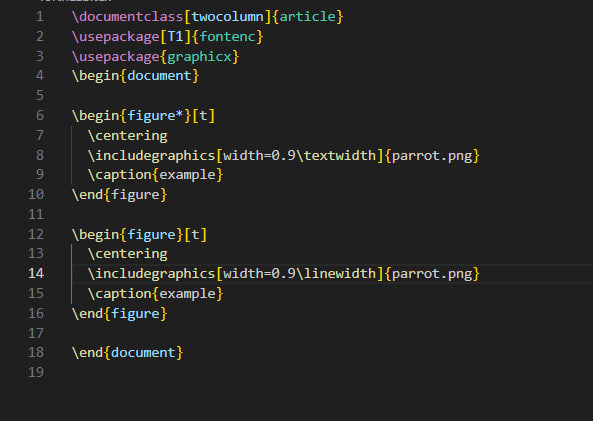
\includegraphics[width=0.7\linewidth,height=\textheight,keepaspectratio]{image/23.jpg}

}

\caption{\label{fig-023}Две колонки}

\end{figure}%

Здесь мы видим, что у изображений разный размер. Так как второе
расположено в одной из двух колонок.

\begin{figure}

\centering{

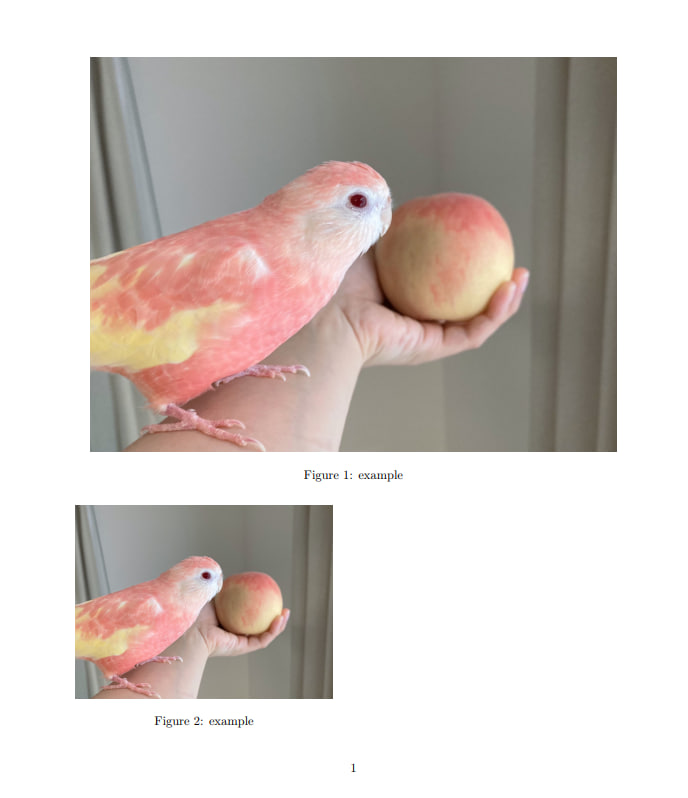
\includegraphics[width=0.7\linewidth,height=\textheight,keepaspectratio]{image/24.jpg}

}

\caption{\label{fig-024}Явные различия}

\end{figure}%

Здесь смотрим как выглядят типы расположения объектов.

\begin{figure}

\centering{

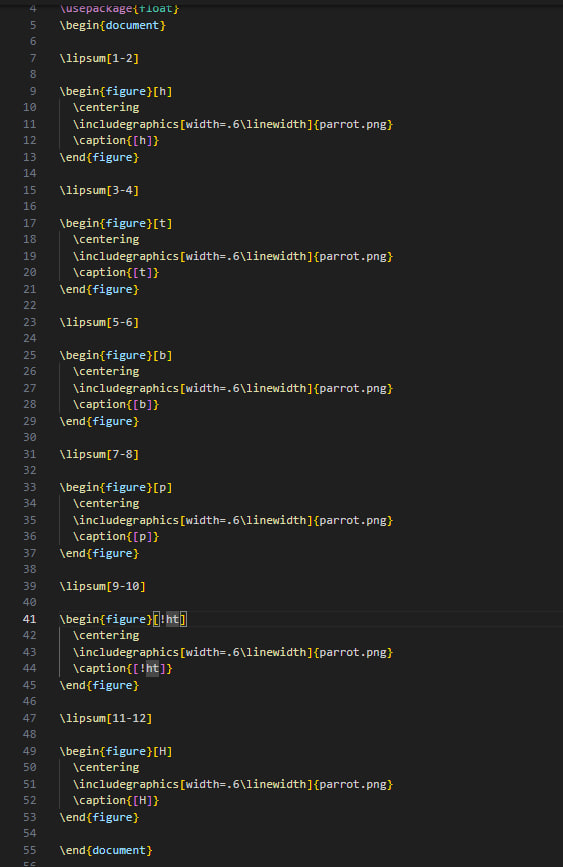
\includegraphics[width=0.7\linewidth,height=\textheight,keepaspectratio]{image/25.jpg}

}

\caption{\label{fig-025}Спецификаторы}

\end{figure}%

\begin{figure}

\centering{

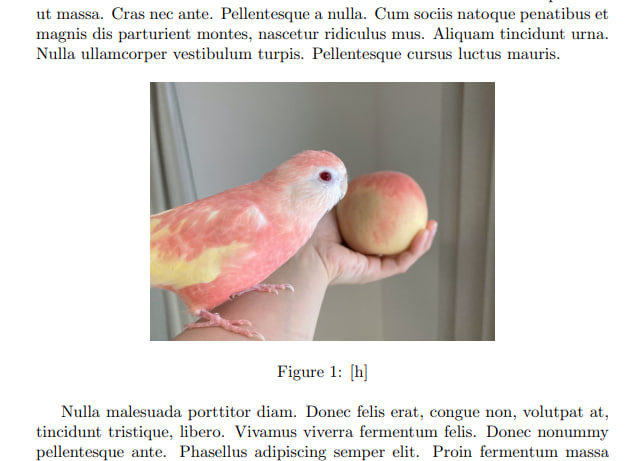
\includegraphics[width=0.7\linewidth,height=\textheight,keepaspectratio]{image/26.jpg}

}

\caption{\label{fig-026}Тип h}

\end{figure}%

Картинки расположились именно так, как мы задали. Но остальные съехали в
конец документа.

\begin{figure}

\centering{

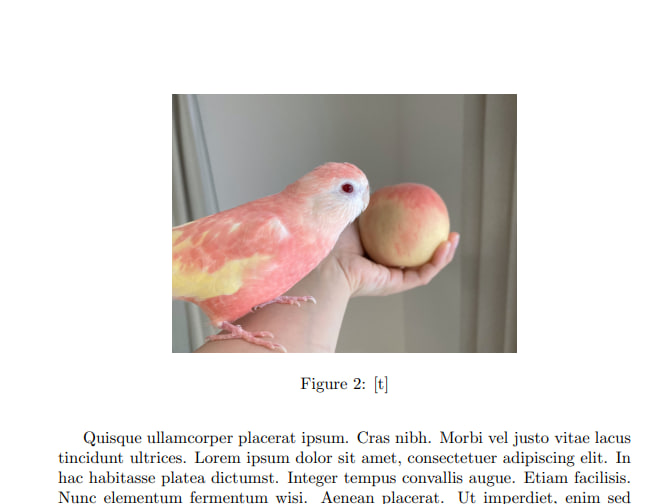
\includegraphics[width=0.7\linewidth,height=\textheight,keepaspectratio]{image/27.jpg}

}

\caption{\label{fig-027}Тип t}

\end{figure}%

Теперь попробуем добавить сами секции, подсекцию и нумерованный список.
А также сделаем ссылки.

\begin{figure}

\centering{

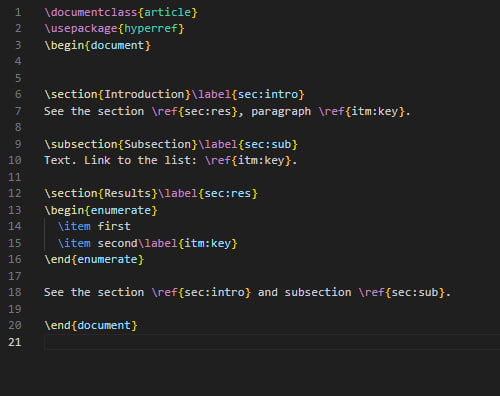
\includegraphics[width=0.7\linewidth,height=\textheight,keepaspectratio]{image/28.jpg}

}

\caption{\label{fig-028}Новые секции}

\end{figure}%

\begin{figure}

\centering{

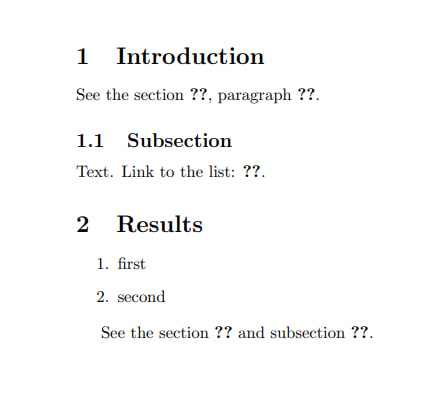
\includegraphics[width=0.7\linewidth,height=\textheight,keepaspectratio]{image/29.jpg}

}

\caption{\label{fig-029}Результат после первой конвертации}

\end{figure}%

\begin{figure}

\centering{

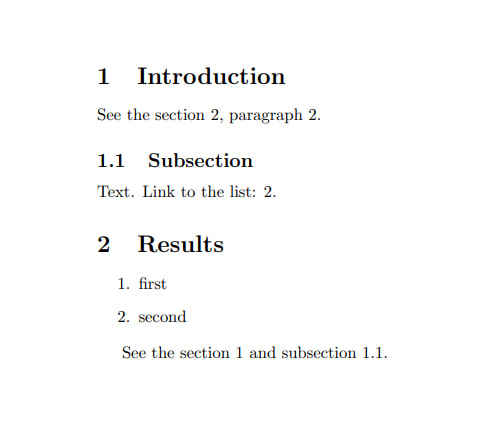
\includegraphics[width=0.7\linewidth,height=\textheight,keepaspectratio]{image/30.jpg}

}

\caption{\label{fig-030}Вторая конвертация}

\end{figure}%

Поробуем расположить label после caption вместо до

\begin{figure}

\centering{

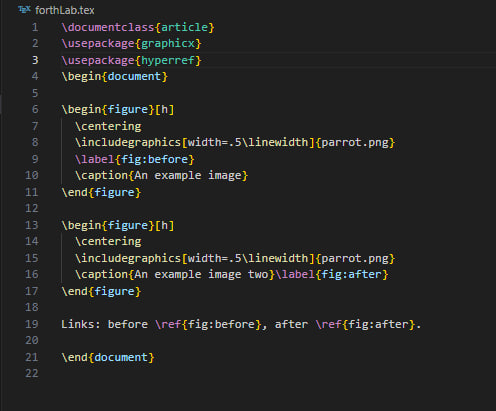
\includegraphics[width=0.7\linewidth,height=\textheight,keepaspectratio]{image/31.jpg}

}

\caption{\label{fig-031}Оба варианта расположения}

\end{figure}%

\begin{figure}

\centering{

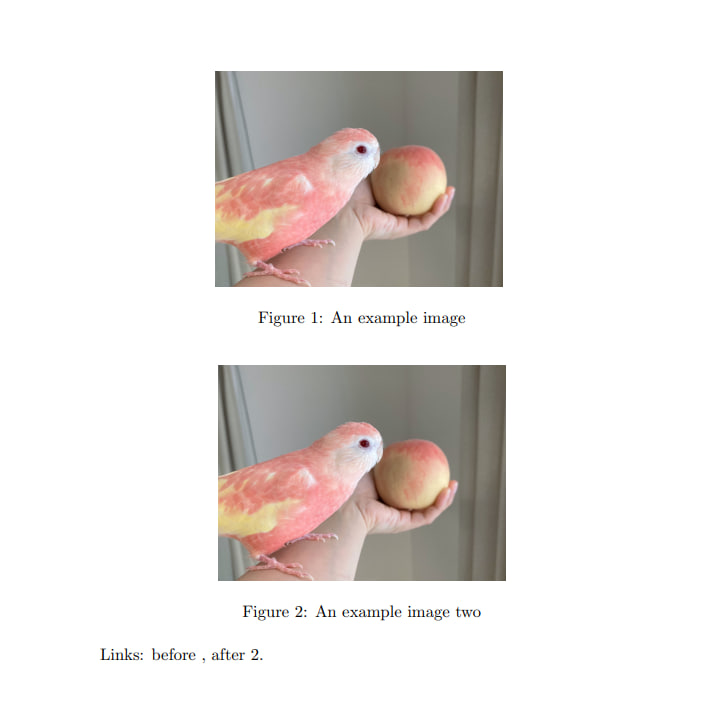
\includegraphics[width=0.7\linewidth,height=\textheight,keepaspectratio]{image/32.jpg}

}

\caption{\label{fig-032}Результат неправильного названия}

\end{figure}%

И последнее, посмотрим, что будет, если расположить label для уравнения
после end\{equation\}?

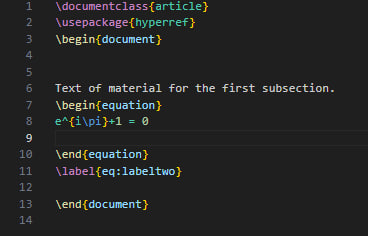
\includegraphics[width=0.7\linewidth,height=\textheight,keepaspectratio]{image/33.jpg}

\includegraphics[width=0.7\linewidth,height=\textheight,keepaspectratio]{image/34.jpg}

Мы видим, что нумерация стоит отдельно от уравнения.

\chapter{Выводы}\label{ux432ux44bux432ux43eux434ux44b}

В ходе данной работы мы разобрались, как оформлять изображения в тексте,
изменять их, а также, как правильно работать с ссылками.

\chapter*{Список
литературы}\label{ux441ux43fux438ux441ux43eux43a-ux43bux438ux442ux435ux440ux430ux442ux443ux440ux44b}
\addcontentsline{toc}{chapter}{Список литературы}

\printbibliography[heading=none]





\end{document}
